\section{Methodology}
In this section you should describe the method of the experiment.



\subsection{Hardware}
The experiments conducted in this report were performed on a computer with the following specifications:
\begin{itemize}
	\item CPU: i5-2500 (4 cores @ 3.3-3.7	GHz)
	\item RAM: 8 GB DDR3
	\item OS:  Ubuntu 15.04
\end{itemize}

\subsection{Introductory Experiments}
To breed foster familiarity with Octave, a task was issued that involved generating a .wav file with a given method, and then creating one for comparison. The difference between the two functions being that the first one relies on a single call to rand() to generate multiple values, while the new method makes a call to rand() for each value in turn. A sample rate of 8000Hz was used, to decrease computation time. 

The given implementation took 173ms to generate 1000s of 8000Hz white noise. The custom implementation took 64244ms. This new method is a handy 370 times slower than the original method. This speed-down is likely due to the overheads of calling the rand() function multiple times.

The code for the custom implementation is shown below:

\begin{Matlab}
function whiten = createwhiten(time)
  sample_rate = 8000;
  whiten = zeros(time*sample_rate,1);
  samples = time*sample_rate
  for i = 1:samples
    whiten(i) = rand();
  end
  
  whiten = whiten*2-1; %fit into .wav bounds
end
\end{Matlab}


\subsection{Custom Correlation Implementation}
The source code for the bespoke correlation solution is shown below.

\begin{Matlab}
function r = mycorr(x,y)
	% readability >> succinctness
	sx  = sum(x);
	sy  = sum(y);
	sxy = sum(x.*y);    % elementwise multiplication
	sx2 = sum(x.^2);    % elementwise squares
	sy2 = sum(y.^2);
	n   = max(size(x)); % just in case we get some column/row vector mixups
	num = sxy - sx*sy/n;
	den = sqrt((sx2-(sx.^2)/n)*(sy2-(sy.^2)/n));
	r = -2; % default, in case correlation could not be performed
	if(den != 0)
		r = num/den;
	end
end
\end{Matlab}

\subsection{Comparing Signals Shifted in Time}

Firstly, a signal must be generated, and then compared against a shifted version of itself. This can easily be done by generating a signal and then using a small 'window' of the signal compared to a window shifted slightly to either side, i.e. if the signal x is comprised of 100 samples, one signal could be x[1:50] and the shifted version 20 samples ahead, at x[21:70]. For all instances, I used a window size of 50 samples.

The signals generated were simple sine waves, at frequencies of 1rad/s, 2rad/s, and 10rad/s. All of the signals generated range from -pi to pi (shown in Figure~\ref{fig:overview}). 100, 1000, and 10000 samples were used for each frequency.  The choice of windows are [1:50] (the first 50 samples of the signal), [2:51] (a shift by 1), and [11:61] (a shift by 10). 

These values were chosen to cover a wide range of signals, and to avoid jumping to conclusions.

Figure~\ref{fig:windowslo100} shows a low frequency, low sample rate signal viewed through the different windows. Figure~\ref{fig:windowshi100} shows a high frequency, low sample rate signal viewed through the different windows. Figure~\ref{fig:windows10000} shows a high frequency, high sample rate signal viewed through the different windows. Figure~\ref{fig:absvals} shows the absolute value of the differences between shifted signals at different sample rates.

Judging from these figures the inference can be drawn that low sample rate signals will be more heavily affected by a shift in samples, as there is a larger gap of information between each sample. 

The correlation between each signal was calculated using the native corr function as follows:

\begin{Matlab}
a = linspace(-pi,pi,100); %100 samples
x1  = sin(a*1); %frequency of 1rad/s
w1 = 1:50;
w2 = 2:51;
r = corr(x1(w1),x1(w2));
disp(r);
\end{Matlab}

\begin{figure}
\centering
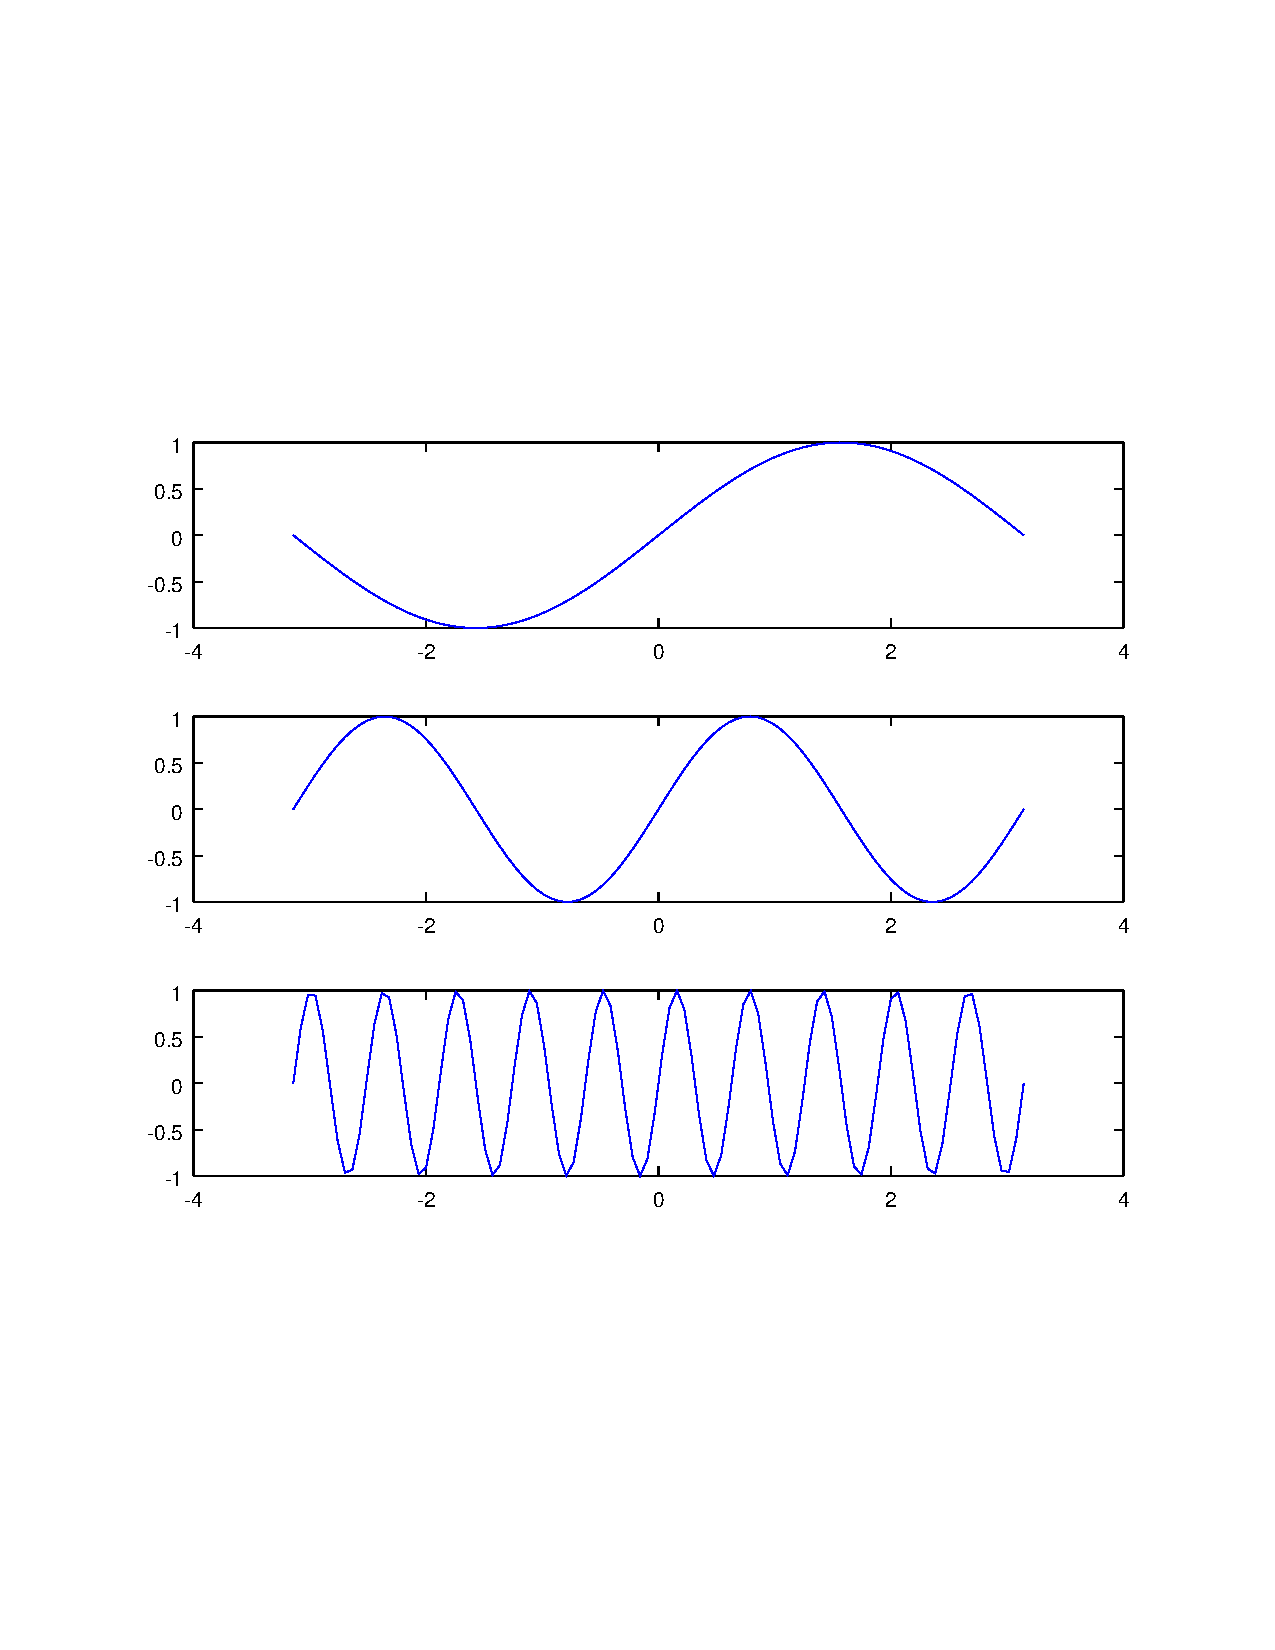
\includegraphics[scale=0.4]{Figures/overview}
\caption{Overview of signals}
\label{fig:overview}
\end{figure}


\begin{figure}
\centering
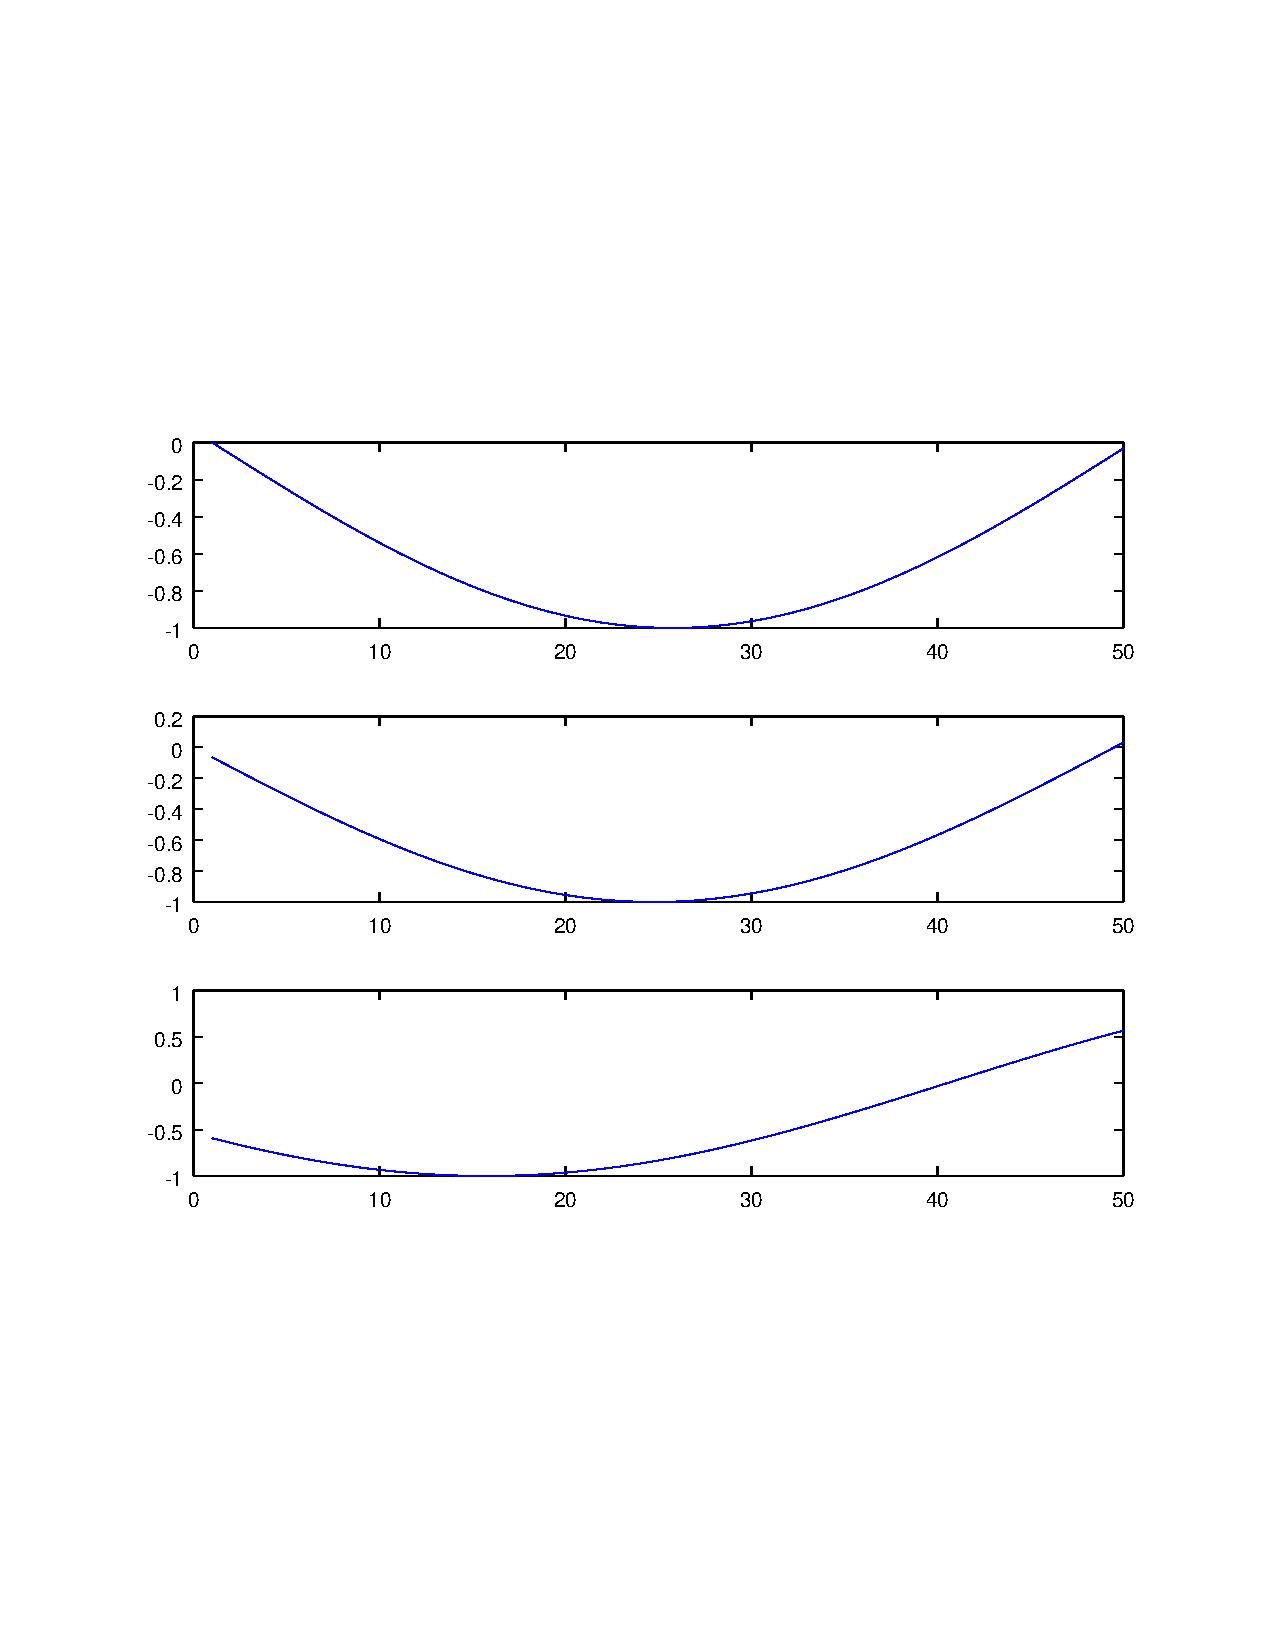
\includegraphics[scale=0.4]{Figures/lofreq}
\caption{Overview of signals}
\label{fig:windowslo100}
\end{figure}

\begin{figure}
\centering
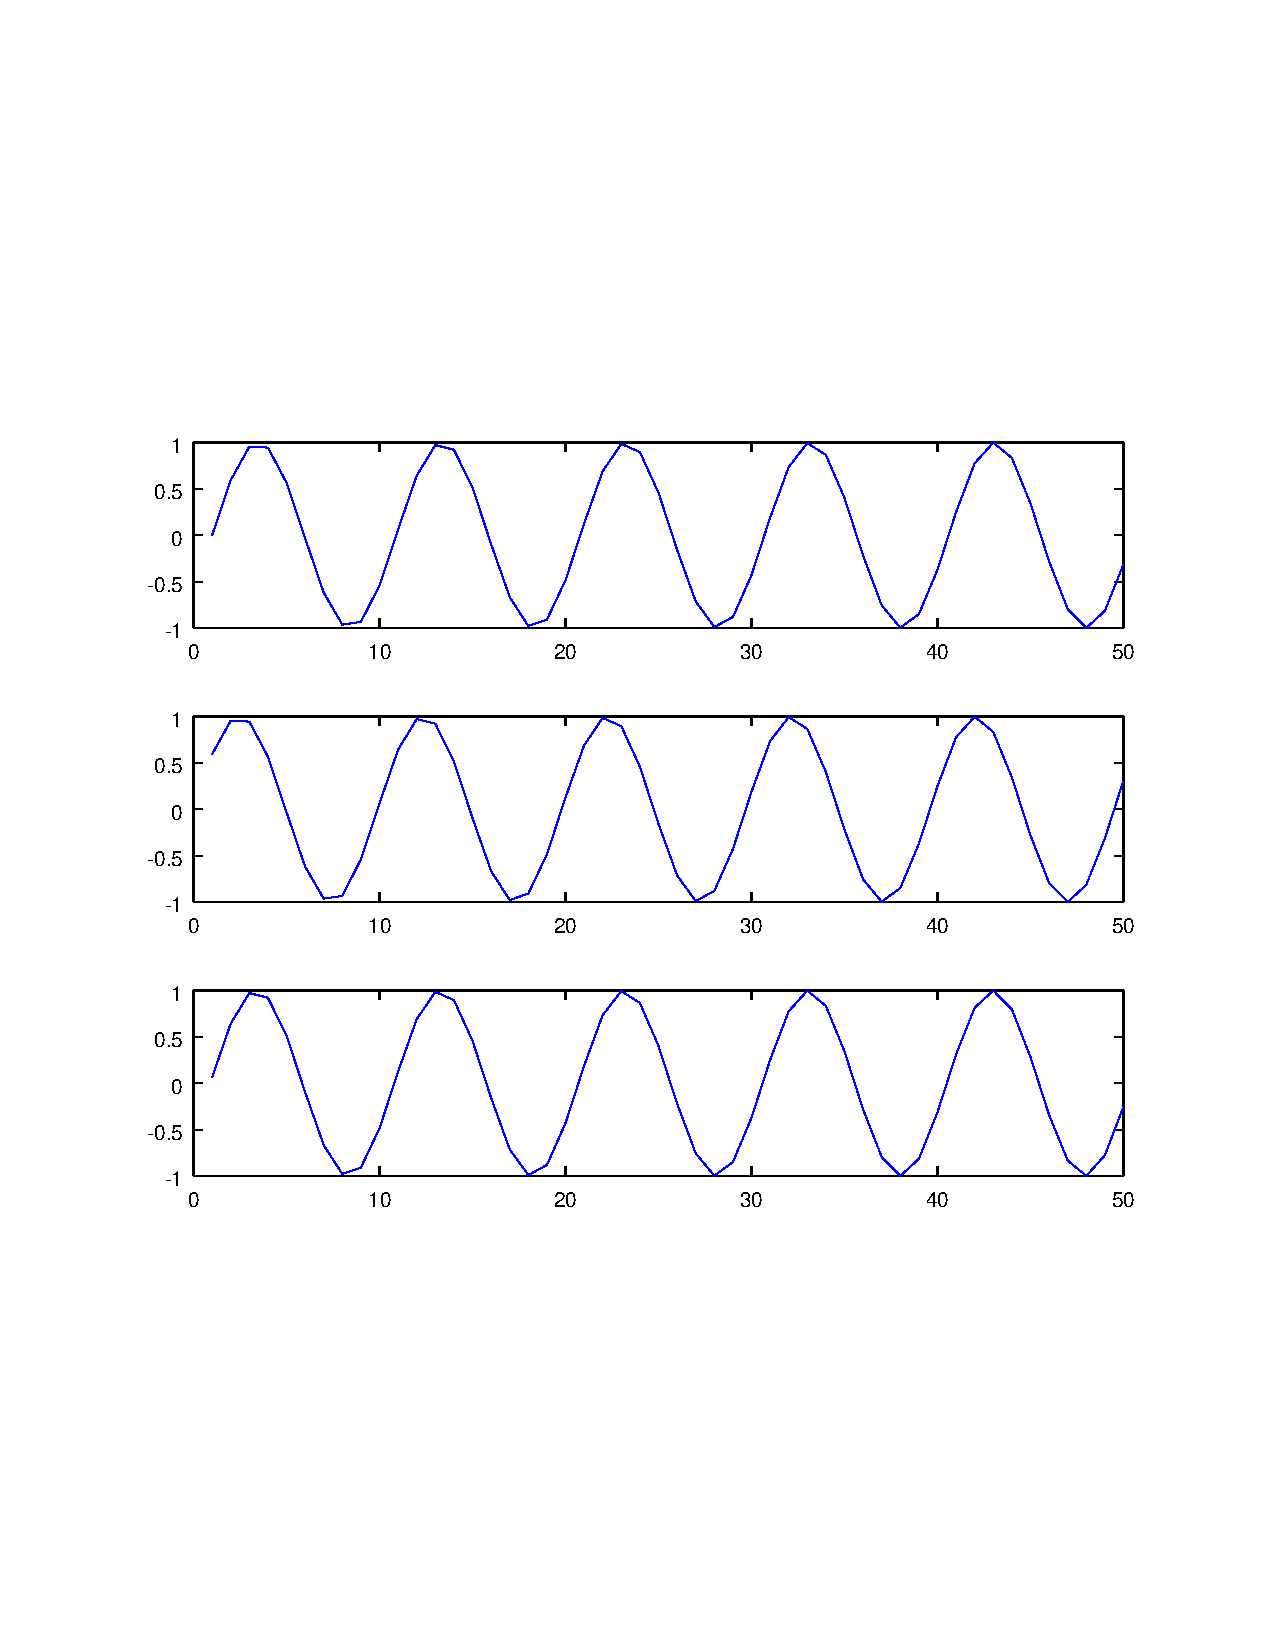
\includegraphics[scale=0.4]{Figures/hifreq}
\caption{Overview of signals}
\label{fig:windowshi100}
\end{figure}

\begin{figure}
\centering
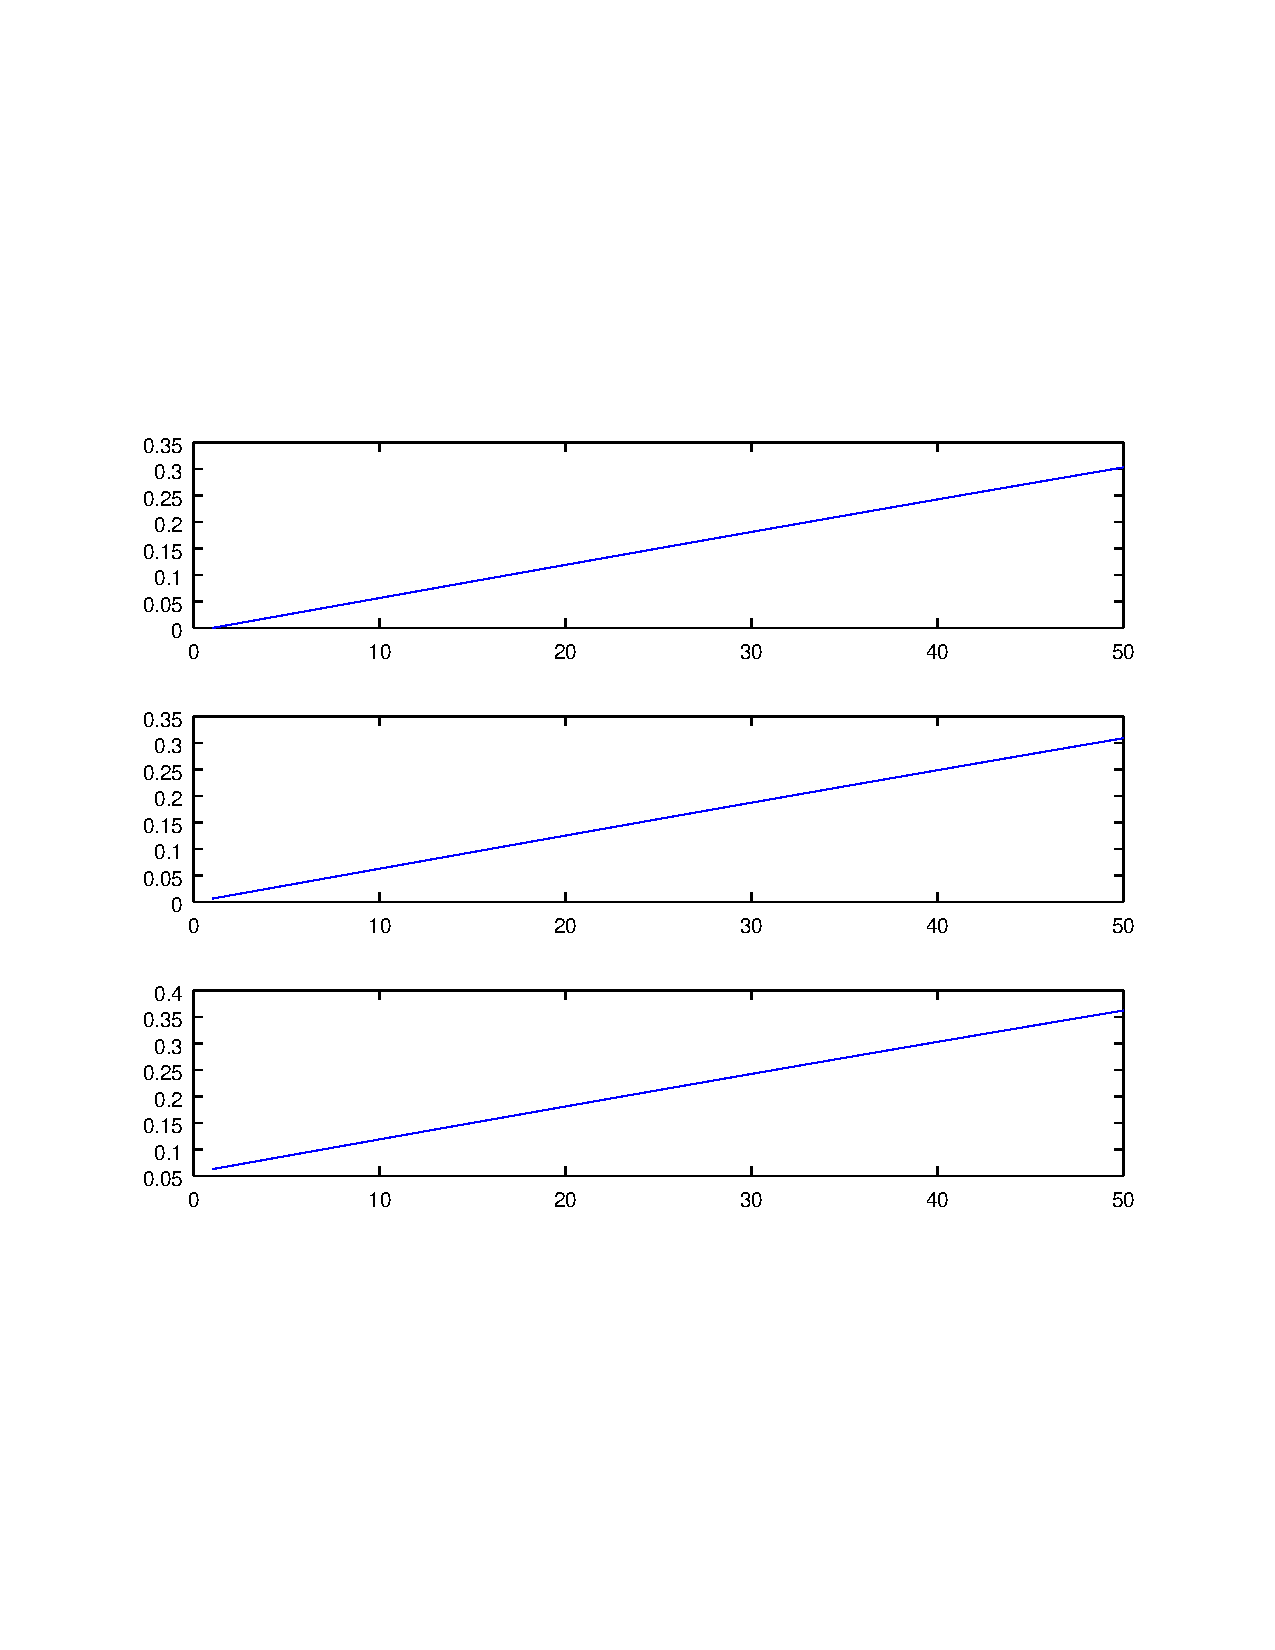
\includegraphics[scale=0.4]{Figures/hifreqhisample}
\caption{Overview of signals}
\label{fig:windows10000}
\end{figure}

\begin{figure}
\centering
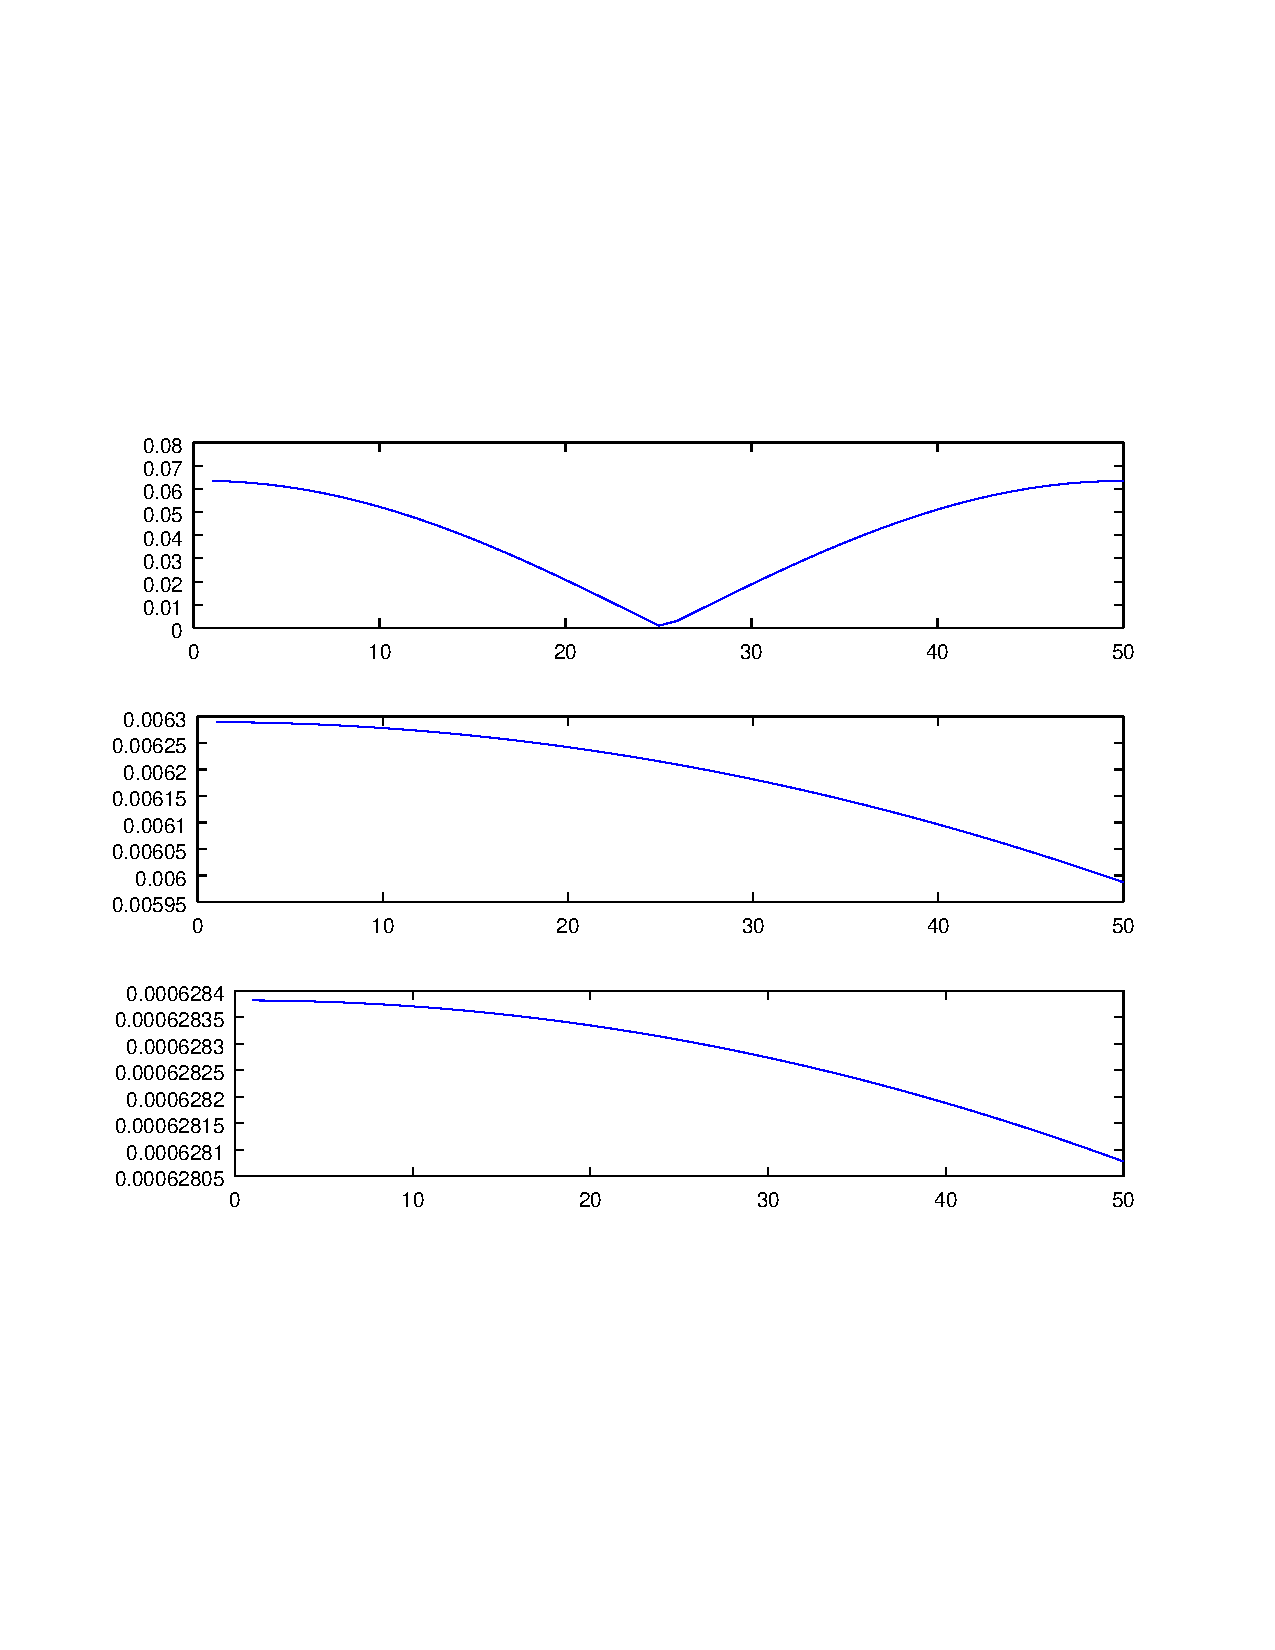
\includegraphics[scale=0.4]{Figures/absvals}
\caption{Overview of signals}
\label{fig:absvals}
\end{figure}



\subsection{Experiment Procedure}
Furthermore, include detail relating to the experiment itself: what did you do, in what order was this done, why was this done, etc.  What are you trying to prove / disprove?